\chapter{Посібник користувача}
\label{app:user_manual}

\section{Вступ}
\label{sec:manual_intro}
Цей посібник користувача надає інструкції щодо використання основних функцій веб-платформи для комунікації та обміну знаннями в спільноті бджолярів \textit{Beekeepers Community Platform}. Він призначений для допомоги новим та існуючим користувачам у навігації та ефективному використанні доступних інструментів для управління пасікою, обміну досвідом та взаємодії з іншими учасниками спільноти.

\section{Реєстрація та вхід до системи}
\label{sec:manual_auth}

\subsection{Реєстрація нового користувача}
\label{subsec:manual_registration}
Для створення нового облікового запису на платформі, що відкриє Вам доступ до всіх її можливостей, виконайте наступні кроки:
\begin{enumerate}
    \item Перейдіть на сторінку реєстрації. Зазвичай посилання на неї знаходиться на головній сторінці або сторінці входу.
    \item Уважно заповніть форму реєстрації, вказавши Вашу актуальну електронну адресу (вона буде використовуватись для входу та отримання сповіщень), бажане ім\'я користувача (username), яке буде відображатися іншим учасникам платформи, та надійний пароль (див. рисунок \ref{fig:manual_registration_form}). Рекомендується використовувати комбінацію літер, цифр та спеціальних символів для підвищення безпеки Вашого пароля.
    \item Натисніть кнопку "Зареєструватися" для відправки даних.
    \item Після успішної реєстрації, система автоматично надішле електронний лист на вказану Вами адресу для підтвердження її автентичності. Відкрийте цей лист (перевірте також папку "Спам", якщо лист не надійшов протягом кількох хвилин) та перейдіть за унікальним посиланням для активації Вашого облікового запису. Цей крок є надзвичайно важливим для забезпечення безпеки та підтвердження, що саме Ви є власником вказаної електронної пошти.
\end{enumerate}

\begin{figure}[htbp]
    \centering
    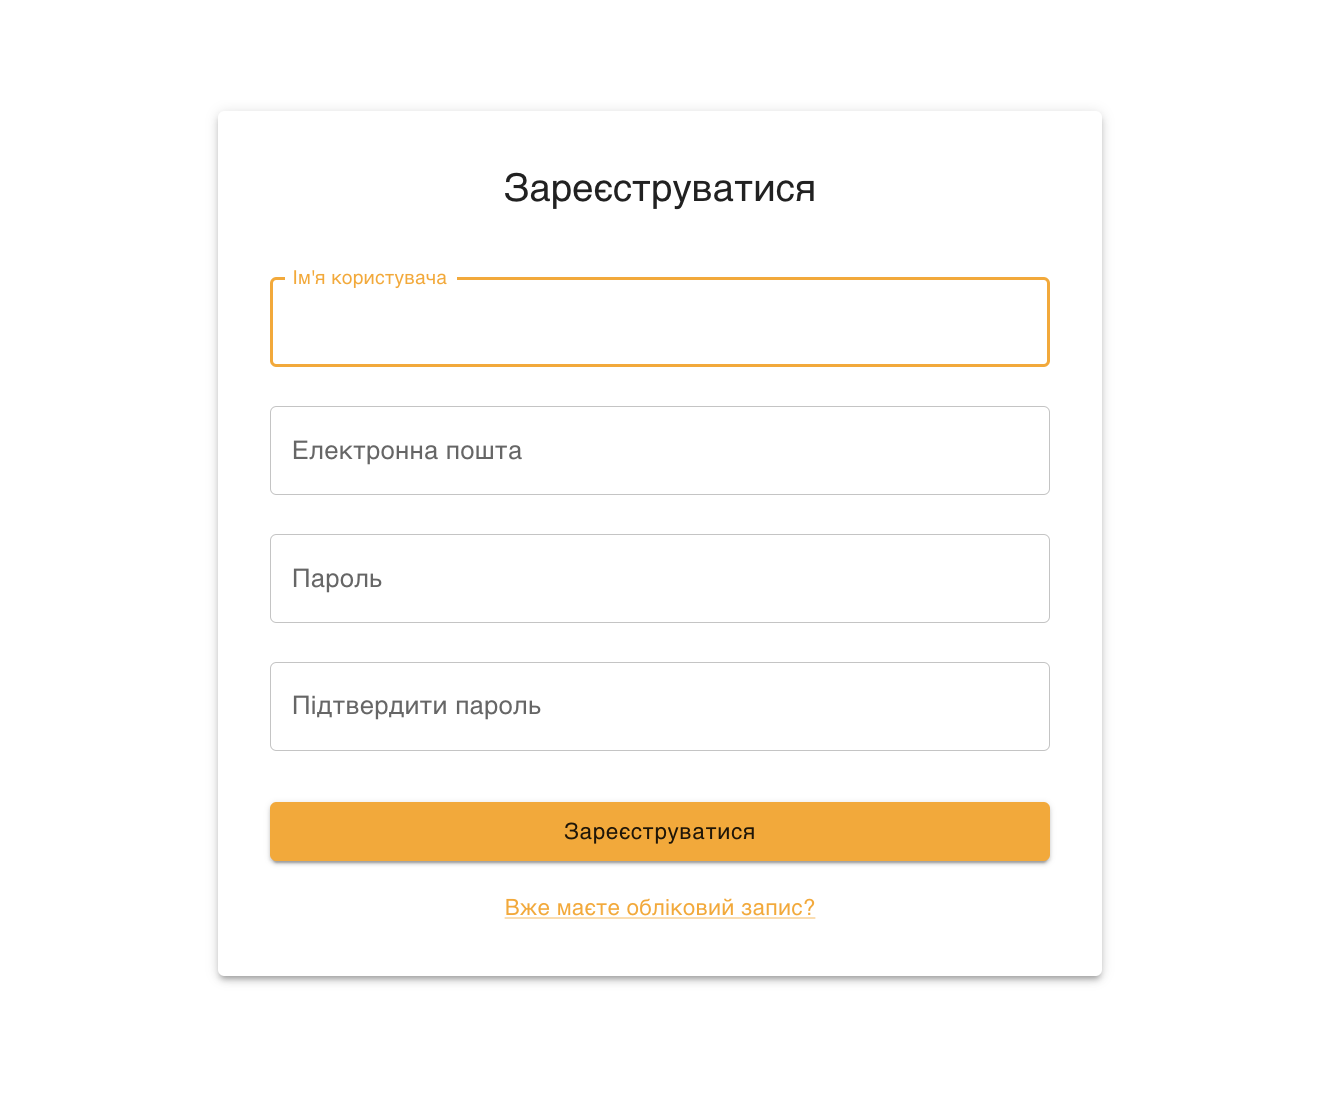
\includegraphics[width=0.6\textwidth]{practice_report/images/registration_form.png}
    \caption{Форма реєстрації нового користувача (Посібник)}
    \label{fig:manual_registration_form}
\end{figure}

% TODO: Add text and screenshot for email verification page/prompt (e.g., VerifyEmailPage.tsx screenshot)

\subsection{Вхід до системи}
\label{subsec:manual_login}
Для входу до системи, якщо у Вас вже є активний обліковий запис:
\begin{enumerate}
    \item Перейдіть на сторінку входу, яка зазвичай є стартовою сторінкою платформи для неавторизованих користувачів (див. рисунок \ref{fig:manual_login_page}).
    \item Введіть Вашу електронну адресу та пароль, вказані при реєстрації, у відповідні поля.
    \item Натисніть кнопку "Увійти". У разі успішної автентифікації, Ви будете перенаправлені на головну сторінку платформи або Ваш особистий кабінет.
    \item Альтернативно, якщо Ви раніше пов\'язали свій обліковий запис або бажаєте зареєструватися через Google, Ви можете увійти за допомогою свого облікового запису Google, натиснувши відповідну кнопку. Це дозволить швидко автентифікуватися без необхідності введення пароля.
\end{enumerate}

\begin{figure}[htbp]
    \centering
    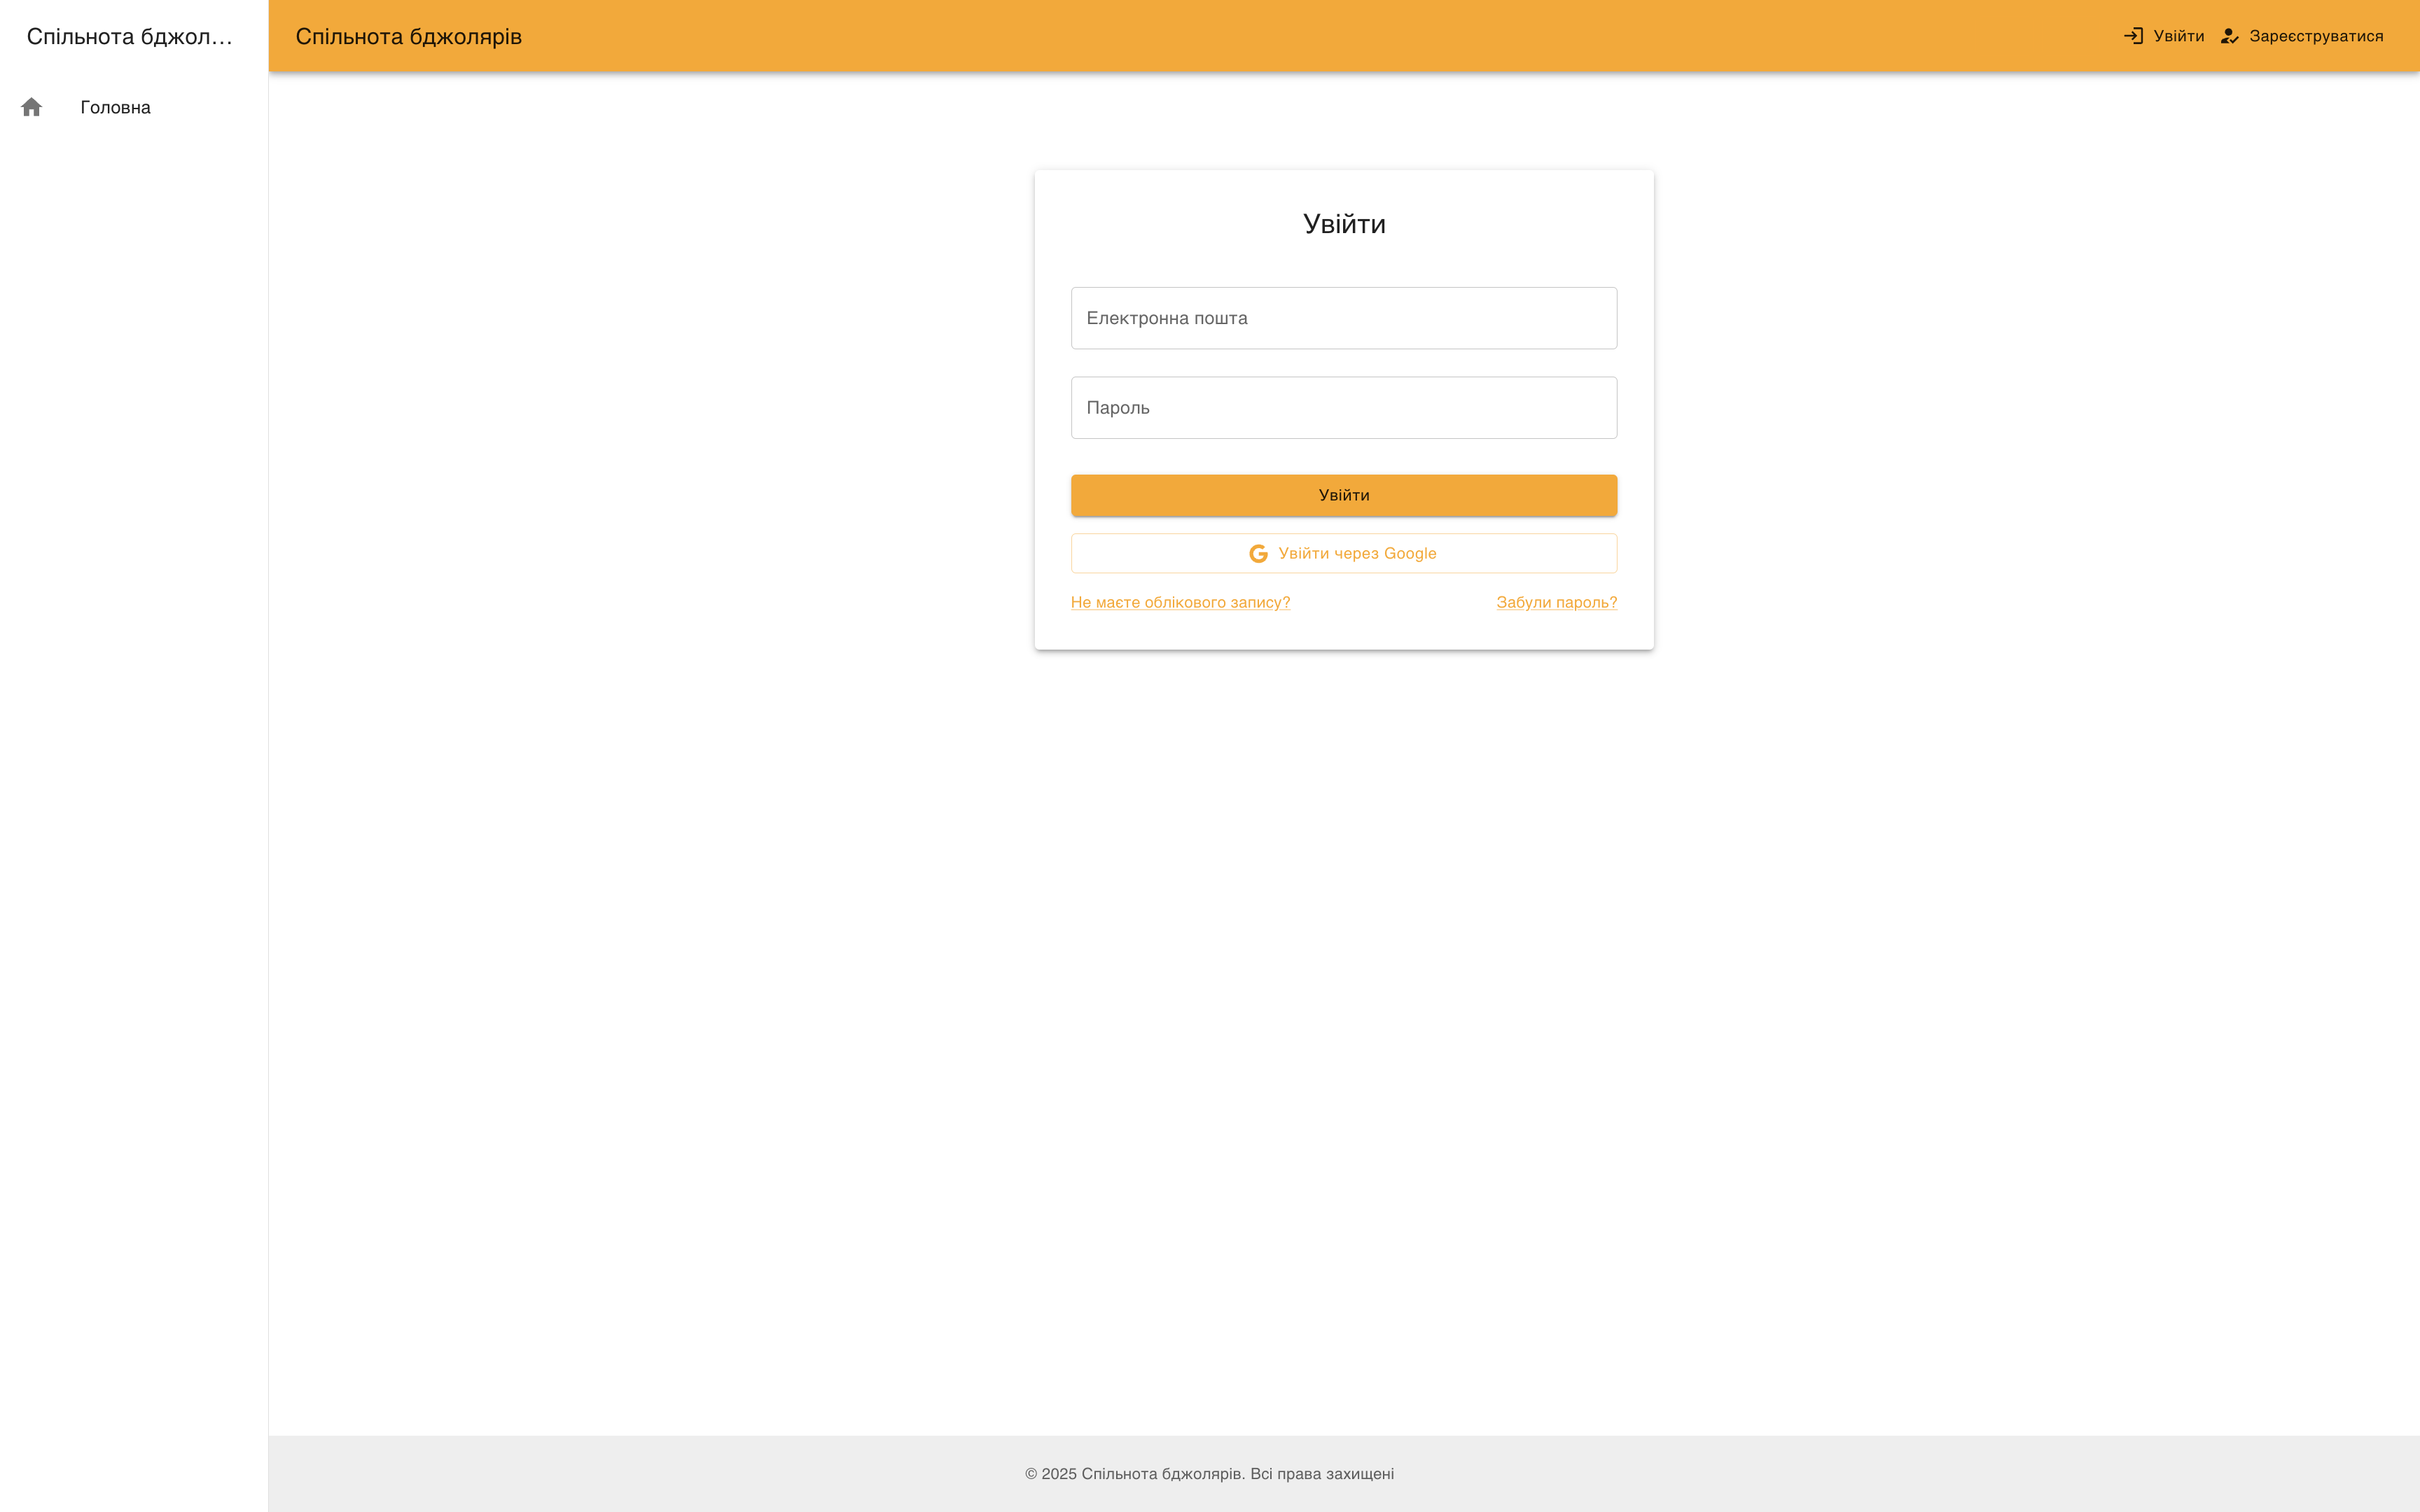
\includegraphics[width=0.6\textwidth]{practice_report/images/login_page.png}
    \caption{Сторінка входу до системи (Посібник)}
    \label{fig:manual_login_page}
\end{figure}

% TODO: Add text and screenshot for what happens after successful login (e.g., dashboard or main page view)

\section{Використання інтерактивної карти}
\label{sec:manual_map}

\subsection{Огляд інтерфейсу карти}
% TODO: General description of the map interface, perhaps a full-view screenshot if different from specific demos.
Карта надає візуальний інтерфейс для управління вуликами та полями. На ній відображаються маркери вуликів та полігони полів, а також елементи керування для додавання нових об\'єктів та навігації. Ви можете масштабувати карту та переміщатися по ній для огляду різних територій.

\subsubsection{Перегляд вуликів}
\label{subsec:manual_map_hives}
Інтерактивна карта дозволяє переглядати розташування Ваших вуликів, а також вуликів інших користувачів, якщо це передбачено налаштуваннями приватності. Кожен вулик позначений спеціальною тематичною іконкою для легкої ідентифікації. При натисканні на маркер вулика з\'являється спливаюче вікно (popup), яке надає детальну інформацію про вулик, таку як його назва, опис, дата створення, та можливо, інша специфічна інформація, додана власником. У цьому ж вікні зазвичай знаходяться кнопки для можливих дій, наприклад, видалення вулика (якщо Ви є його власником) або перехід до сторінки з більш детальною інформацією (див. рисунок \ref{fig:manual_map_hives_demo}).

\begin{figure}[htbp]
    \centering
    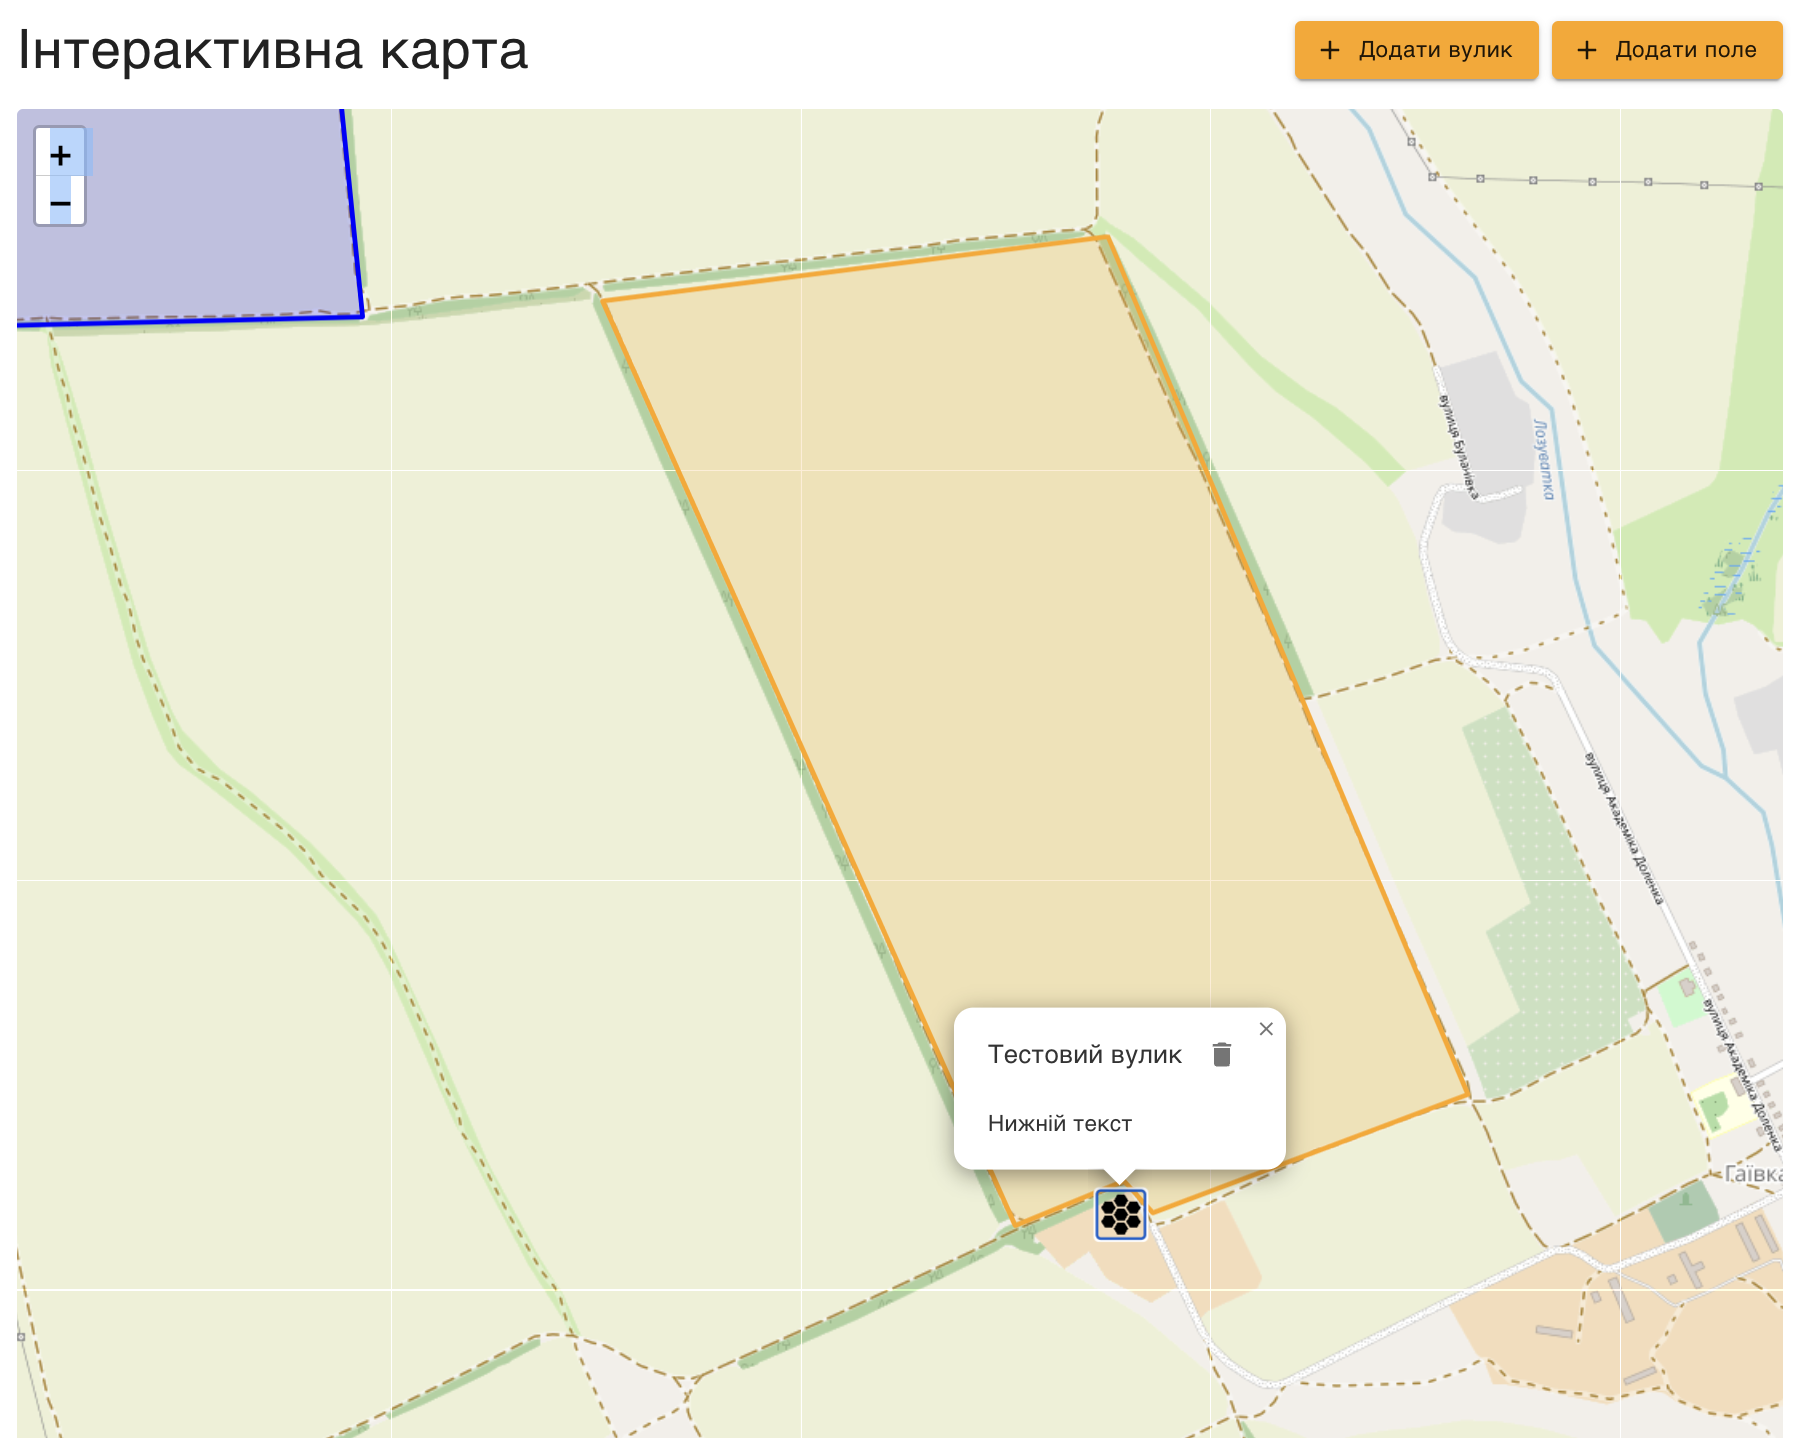
\includegraphics[width=0.8\textwidth]{practice_report/images/map_hives_demo.png}
    \caption{Відображення вуликів на карті з інформаційним вікном (Посібник)}
    \label{fig:manual_map_hives_demo}
\end{figure}

% TODO: Add sections for Adding Hives, Deleting Hives with relevant screenshots/dialogs.

\subsubsection{Перегляд полів}
\label{subsec:manual_map_fields}
Аналогічно до вуликів, Ви також можете переглядати інформацію про сільськогосподарські поля, які позначені на карті полігонами, що відображають їхні межі. Натискання на полігон поля відкриває спливаюче вікно з його ключовими характеристиками: назва поля, тип вирощуваної культури, орієнтовний період цвітіння та, що особливо важливо, список запланованих дат обробки хімікатами. Колір полігону може динамічно змінюватися для візуальної індикації нещодавніх або майбутніх обробок, що допомагає бджолярам оцінити потенційні ризики для своїх бджіл. У спливаючому вікні також доступні кнопки управління, наприклад, для редагування даних поля, якщо Ви маєте відповідні права (див. рисунок \ref{fig:manual_map_fields_demo}).

\begin{figure}[htbp]
    \centering
    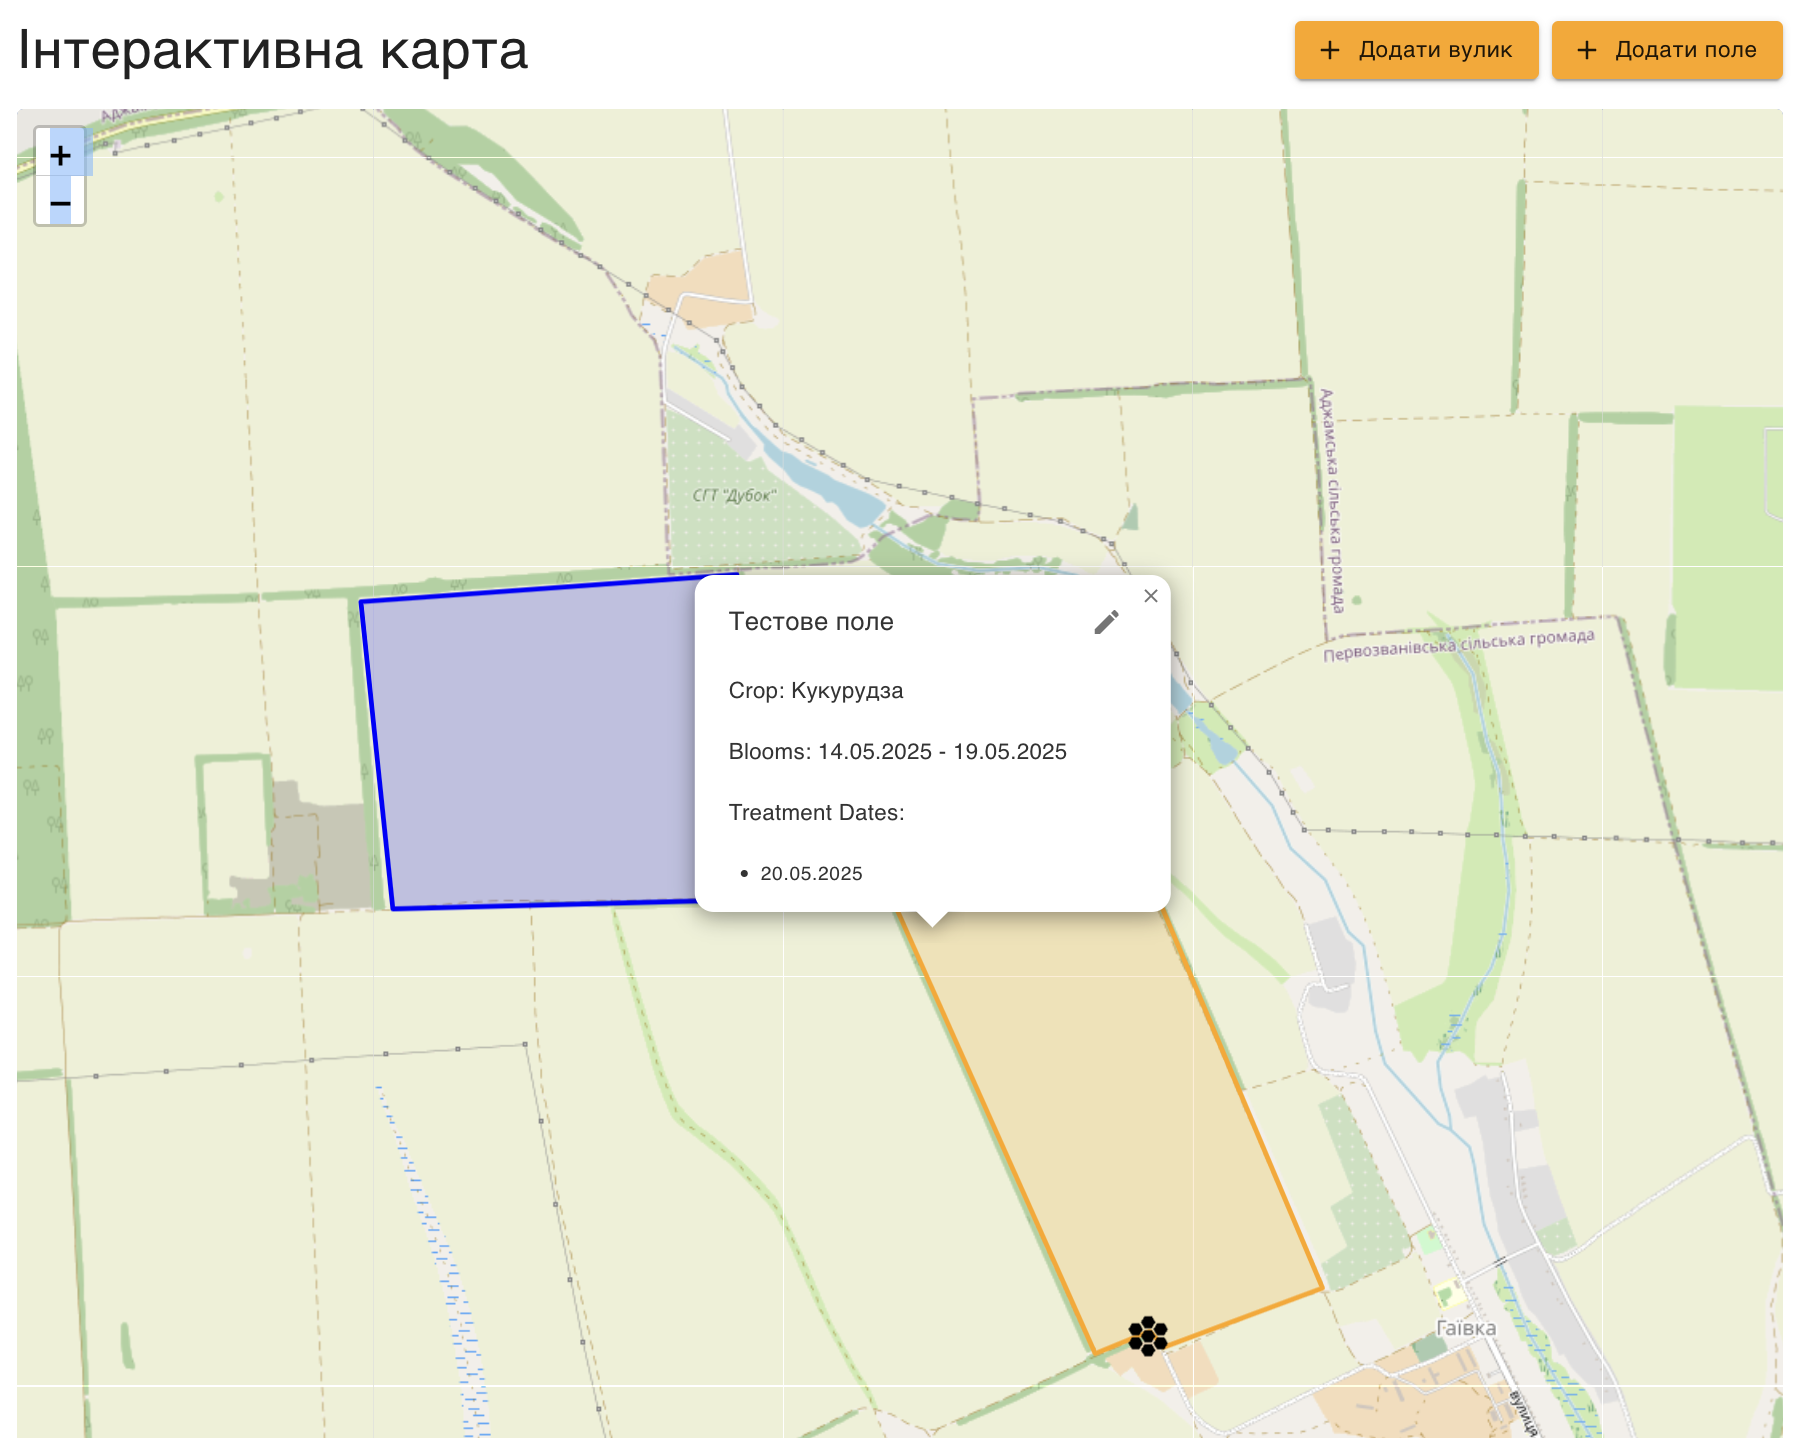
\includegraphics[width=0.8\textwidth]{practice_report/images/map_fields_demo.png}
    \caption{Відображення полів на карті з інформаційним вікном (Посібник)}
    \label{fig:manual_map_fields_demo}
\end{figure}

% TODO: Add sections for Adding Fields, Editing Fields, Deleting Fields with relevant screenshots/dialogs.

% TODO: Add sections for User Profile Management, Forum Usage, Knowledge Base, Admin Panel (if applicable) 